% !TEX root = ../main.tex

\section{Preliminaries}

\subsection{How the \textit{multiple withdrawal attack} works}

According to the ERC20 API definition, the \texttt{approve} function\footnote{We use the term method and function interchangeably.}
allows a spender (\eg user, wallet or other smart contracts) to withdraw up to an allowed amount of tokens from token pool of the approver. If this function is called again, it overwrites the current allowance with the new input value. On the other hand, the \texttt{transferFrom} function allows the spender to actually transfer tokens from the approver to anyone they choose (importantly: not necessarily themselves). The contract updates balance of transaction parties accordingly. 

An adversary can exploit the gap between the confirmation of the \texttt{approve} and \texttt{transferFrom} functions since the \texttt{approve} method replaces the current spender allowance with the new amount, regardless of whether the spender already transferred any tokens or not. This functionality of the \texttt{approve} method is shaped by the language of the standard and cannot be changed. Furthermore, while variables change and events are logged, this information is ambiguous and cannot fully distinguish between possible traces. Consider the following illustration:

\begin{compactlistn}
	\item Alice allows Bob to transfer N tokens on her behalf by broadcasting \texttt{approve(\_Bob, N)}.
	\item Later, Alice decides to change Bob's approval from N to M  by calling \texttt{approve(\_Bob, M)}.
	\item Bob notices Alice's second transaction after it is broadcast to the Ethereum network but before it is added to a block.
	\item Bob front-runs (using an asymmetric insertion attack~\cite{eskandari2019sok}) the original transaction with a call to   \texttt{transferFrom(\_Alice, \_Bob, N)}. If a miner is incentivized (\eg by Bob offering high gas) to add this transaction before Alice's, it will transfer N of Alice's tokens to Bob.
	\item Alice's transaction will then be executed which changes Bob's approval to M.
	\item Bob can call \texttt{transferFrom} method again and transfer M additional tokens by broadcasting \texttt{transferFrom(\_Alice, \_Bob, M)}.
\end{compactlistn}

\begin{figure}[ht]
	\centering
	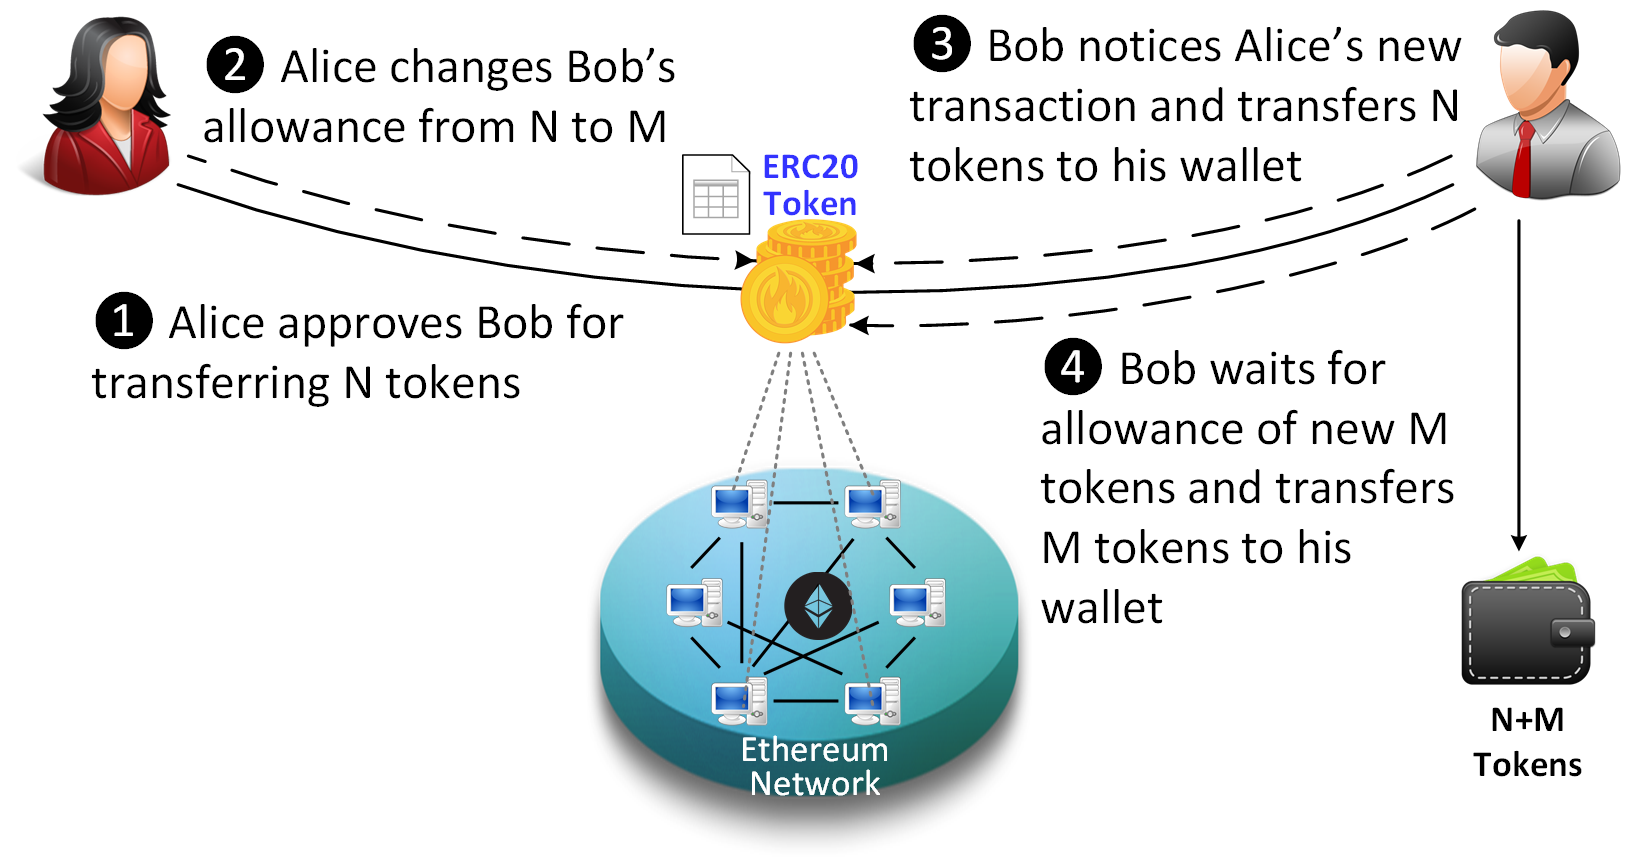
\includegraphics[width=1.0\linewidth]{figures/multiple_withdrawal_02.png}
	\caption{Possible multiple withdrawal attack in ERC20 tokens when Alice changes Bob's allowance from N to M. By front-running, Bob is able to move N+M tokens from token pool of Alice. Solutions should consider Bob's initial transfer of N tokens (step 3) to be legitimate and try to prevent the second transfer of the additional M tokens (step 4).\label{fig:mwa}}
\end{figure}

In summary, in attempting to change Bob's allowance from N to M, Alice makes it possible for Bob to transfer N+M of her tokens. We operate on the assumption that a secure implementation would prevent Bob from withdrawing Alice's tokens multiple times when the allowance changes from N to M (see Figure~\ref{fig:mwa}).

\subsection{Why mitigation is important}

ERC20 tokens are important component of Ethereum's supplementary financial system that have many financial (as well as non-financial) uses and could hold considerable value (potentially exceeding the value of Ether itself). There has been more than 64,000 functional ERC20 tokens as of early 2019~\cite{victormeasuring} that might be vulnerable to this attack. Furthermore, ERC20 tokens that have already been issued cannot easily migrate to a new secure implementation and should these tokens appreciate in value in the future. Resolving the attack also serves as basis for other extended standards, such as ERC-223, ERC-621, and even ERC-777 to be backward compatible with ERC20 interface~\cite{frowis2018detecting} while offering new enhancements. Finally, firms that hold ERC20 tokens require assurance of their security, particularly in the case that they require their financial statements to be audited---an issue like this could lead to further hesitation by auditors.

\subsection{Where to prevent this attack}

There are a few logical places to address this attack. Ideally the token author (instead of the token holders) would mitigate the attack within the ERC20 implementation itself. Since two methods are involved in the attack, it could be addressed within the \texttt{approve} and/or \texttt{transferFrom} method. By contrast, token owners have no control over the implementation of the contract and are relegated to mitigating the attack by carefully monitoring the contract around the time allowance changes are made.

%\noindent In general, there would be off-chain and on-chain transaction to consider when proposing solutions. For this paper, off-chain transactions are out of scope. Therefore, concentration will be on on-chain prevention techniques:
%\begin{enumerate}
%	\item \textbf{Prevention by token owner}: Considering owner responsibility to mitigate the attack in UI (\eg Web3.js) instead of contract (\ie Solidity/Vyper).
%	\item \textbf{Prevention by token author}: Smart contract author(s) have to mitigate the attack by securing either \texttt{approve} or \texttt{transferFrom} methods.
%\end{enumerate}

\subsubsection*{Prevention by token holder}
\label{sec:preho}

Consider Alice, a token holder using a web app (\eg a user interface deployed with web3) to adjust Bob's allowance. If this UI is written to the ERC20 standard, Alice will only have \texttt{approve} available to her. The ERC20 authors~\cite{Ref08} advise Alice against directly changing Bob's allowance from N to M. Instead, she should set the approval to 0 and then it to M. Presumedly, Alice will not do the second approval (setting it from 0 to M) if she sees that Bob withdraws N tokens before her N to 0 adjustment is confirmed. 

How will Alice know whether Bob withdraws first? The answer depends on how deeply her webapp can monitor the blockchain. One option is to monitor the variable that records Bob's allowance (technically an on-blockchain helper dapp could also do this). However if she sees Bob's allowance at 0 after initiating the first adjustment, it does not tell her that Bob did not withdraw N---both methods result in Bob having an allowance of 0 so either (or both) could have been executed.

Next, she might rely on events passed from the contract to her web3 app. \texttt{Transfer} events as specified in ERC20 will log the transfer parameters (\ie  \texttt{address \_from, address \_to, uint256 \_tokens}). Alice's webapp could filter the events and only display transfers matching her address in the \texttt{\_from} field. The displayed transfers will include any transfer Bob makes, however Bob can provide any address in \texttt{\_to}, not just his own, and the event does not report who authorized the transaction (\ie \texttt{msg.sender}). If Alice has many authorizations, she cannot determine if a transfer was initiated by Bob or someone else she has authorized.\footnote{Even if Bob is listed in \texttt{\_to}, another authorized spender might have transferred tokens to Bob to make Alice believe Bob attempted a multiple withdrawal when he actually did not.} Therefore Alice cannot always unambiguously rely on events to determine Bob did not transfer funds (More details in Section~\ref{sec:enfui}). If Alice's web app is beyond web3 and runs a full node maintaining blockchain state, it could correctly detect and attribute all transfers initiated by Bob. 

The takeaway from all these options is that prevention by token owners has some undesirable properties: (1) it splits adjustments into two transactions, (2) because the first transaction needs to be confirmed before the second is initiated, it takes time to complete, and (3) to precisely mitigate this attack, a heavyweight web app is needed to inspect deeper than variable state changes and events. For these reasons, we concentrate on mitigating the attack in the contract itself. If mitigation at the contract level works, allowances can be adjusted with a single function call from any existing lightweight ERC20 user interface, and no additional monitoring of the contract is necessary. 

% Jeremy: I cut a lot of the text in the next two sections because we will get to all these details in time. The reader at this point in the paper isn't ready for these details, she is just thinking about where to solve the problem. 
	
\subsubsection*{Prevention by token author in \texttt{approve}} The next logical place to tackle multiple withdrawal is in the implementation of the \texttt{approve} method. In particular, an \texttt{approve} implementation might be engineered to fail under the conditions of multiple withdrawal, to adjust the approval amount, treat adjustments as relative offsets from the current amount, or other techniques. As we review the 10 solutions, we will see different proposals along these lines, as well as our own proposal in Section~\ref{sec:proposal1}. For now, we emphasize that adherence to the standard is a core challenge as it unequivocally states that: ``If this function is called again, it overwrites the current allowance with \texttt{\_value}''~\cite{Ref08}. 


%Securing \texttt{approve} method could be a solution and prevent the attack. By using compare and set (CAS) pattern \cite{Ref06}, \texttt{approve} method can change spender allowance from N to M atomically (\ie comparing new allowance with transferred token and set it accordingly). Comparison part of CAS requires knowledge of previously transferred tokens that will reveal any token transfer in case of front-running. Although this is promising approach,  setting new allowance in \texttt{approve} method must satisfy ERC20 constraint that dictates "If this function is called again it overwrites the current allowance with \texttt{\_value}" \cite{Ref08}. This does not allow any adjustments in allowance while it is a prerequisite for securing \texttt{approve} method. 

%SHAYAN: REZA I'm not sure what this example is.

%For example, considering front-running by Bob when Alice changes his allowance form 100 to 110, the \texttt{approve} method can reveal 100 transferred tokens by Bob and has to set Bob allowance to 10 (110-100=10). However, based on ERC20 constraints, it must not adjust the allowance and has to set it literally to 110. Consequently, this allows Bob to transfer 100+110=210 tokens in total. We implemented this approach in~\ref{sec:proposal1} and concluded that securing \texttt{approve} method cannot prevent the attack while adhering constraints of the ERC20 standard.
	
\subsubsection*{Prevention by token author in \texttt{transferFrom}} Recall from Figure~\ref{fig:mwa} that step 4 is the offending function call and it is to \texttt{transferFrom}. If we add new state to the contract to track the number of tokens that have been transferred, we can allow approval to work exactly as specified while interpreting it as a ``lifetime'' allowance. We will explain this in more detail in Section~\ref{sec:proposal2}. 


% Based on ERC20 specifications, "approve functions allows \texttt{\_spender} to withdraw from your account multiple times, up to the \texttt{\_value}". Therefore, spender must not be able to transfer more than allowed tokens. That being said, \texttt{transferFrom} method can prevent transferring of new tokens in case of already transferred tokens up to allowed amount. By comparing transferred tokens in \texttt{transferFrom} method, spender will be restricted to move solely the remaining tokens of his allowance. In case of trying to transfer more tokens than allowed, the transaction fails. For example, Alice's new transaction for increasing Bob allowance from 100 to 110, sets Bob allowance to 110 (\texttt{approve} method sets allowance regardless of transferred tokens). However, \texttt{transferFrom} method prevent the attack by not allowing Bob to transfer more than 10 tokens if he had already transferred 100 tokens. We implemented this approach in~\ref{sec:proposal2} and it mitigates the attack effectively.

\subsection{What an ideal solution looks like}
\label{sec:criteria}

We prioritize adherence to the ERC20 standard. While deviating from the standard might become acceptable if there is no possible way to conform with it and maintain security, we consider that a last resort. Indeed, as we will show, it is possible to secure an ERC20 contract within the constraints of the standard, which we summarize here~\cite{Ref08}:

\begin{compactlistn}
\item The input to \texttt{approve} is a new allowance and not a relative adjustment.
\item The result of \texttt{approve} will overwrite the current allowance with the new allowance.
\item A call to \texttt{transferFrom} on an input of 0 tokens will execute as a normal transfer and emit a \texttt{Transfer} event.
\item A spender can call \texttt{transferFrom} multiple times up to the allowed amount.
\item Transferring up to any initial allowance is always a legitimate transfer.
\item An ideal solution cannot rely on overloading existing methods or introducing new methods outside of ERC20, as existing ERC20 dapps and web apps would have to be modified to interoperate.
\item A solution must eliminate all race conditions.
\end{compactlistn}